\chapter{Modelado Funcional y Procesos del Negocio (UML y DFD)}

\section{Modelado de Casos de Uso del Sistema (UML 2.5)}
La interacción entre los actores del negocio y el sistema se estructuró formalmente a través de 15 Casos de Uso (\texttt{CU-01} a \texttt{CU-15}), clasificados en tres actores operacionales:
\begin{itemize}
    \item \textbf{Administrador:} Responsable de la gestión estratégica, catálogos maestros, usuarios, anulación de ventas y reportes gerenciales.
    \item \textbf{Vendedor / Cajero:} Operador de mostrador en tienda física, responsable de ventas, consultas de stock y turnos de caja.
    \item \textbf{Visitante Web (Cliente Final):} Usuario público sin autenticación que consulta el catálogo digital y existencias físicas.
\end{itemize}

\begin{table}[H]
\centering
\small
\begin{tabularx}{\textwidth}{>{\ttfamily\centering}p{1.4cm} >{\raggedright\bfseries}p{4.2cm} >{\raggedright}p{2.6cm} Y}
\toprule
\textbf{Código} & \textbf{Caso de Uso} & \textbf{Actor Primario} & \textbf{Descripción Operacional} \\
\midrule
CU-01 & Iniciar Sesión en el Sistema & Admin, Vendedor & Validación de credenciales con bloqueo preventivo al tercer fallo. \\
CU-02 & Gestionar Usuarios y Roles & Administrador & Alta, baja lógica, modificación, desbloqueo y reseteo de claves. \\
CU-03 & Cerrar Sesión Segura & Admin, Vendedor & Revocación y destrucción de tokens de acceso en el cliente y servidor. \\
CU-04 & Consultar Inventario y Stock & Admin, Vendedor & Búsqueda predictiva y filtros combinados con desglose por sucursal. \\
CU-05 & Registrar y Editar Prendas & Administrador & Alta de prendas, fotos HD, precios y variantes con catálogos cerrados. \\
CU-06 & Ajustar Stock en Kardex & Administrador & Asientos de ingreso de mercadería, mermas o regularización física. \\
CU-07 & Mantener Catálogos Maestros & Administrador & Gestión de Categorías, Marcas, Tallas y Colores (RF-74). \\
CU-08 & Procesar Venta en Mostrador & Vendedor & Terminal POS, carrito, cálculo de totales, cambio y pago mixto. \\
CU-09 & Emitir Ticket Digital & Vendedor & Generación de ticket correlativo, impresión térmica y envío WhatsApp. \\
CU-10 & Sincronizar Ventas Offline & Sistema & Almacenamiento local en IndexedDB y consolidación en lote al conectar. \\
CU-11 & Consultar Historial de Ventas & Admin, Vendedor & Auditoría de tickets emitidos por fechas, local comercial y estado. \\
CU-12 & Anular Venta Comercial & Administrador & Anulación con clave de Admin y restitución atómica de existencias. \\
CU-13 & Generar Reporte de Ventas & Administrador & Métricas de recaudación por fecha, tienda y vendedor con filtros. \\
CU-14 & Analizar Rotación de Productos & Administrador & Ranking Top 10 prendas más vendidas y detección de baja rotación. \\
CU-15 & Explorar Catálogo Web Público & Visitante Web & Galería responsiva sin login con disponibilidad física por tienda. \\
\bottomrule
\end{tabularx}
\caption{Catálogo oficial de los 15 Casos de Uso del sistema SYSELL Web v2.0}
\label{tab:casos_de_uso}
\end{table}

\subsection{Diagrama General de Casos de Uso}
El diagrama general integra las fronteras del sistema, los tres actores clave y los 15 casos de uso agrupados en sus respectivos subsistemas de negocio:

\begin{figure}[H]
\centering
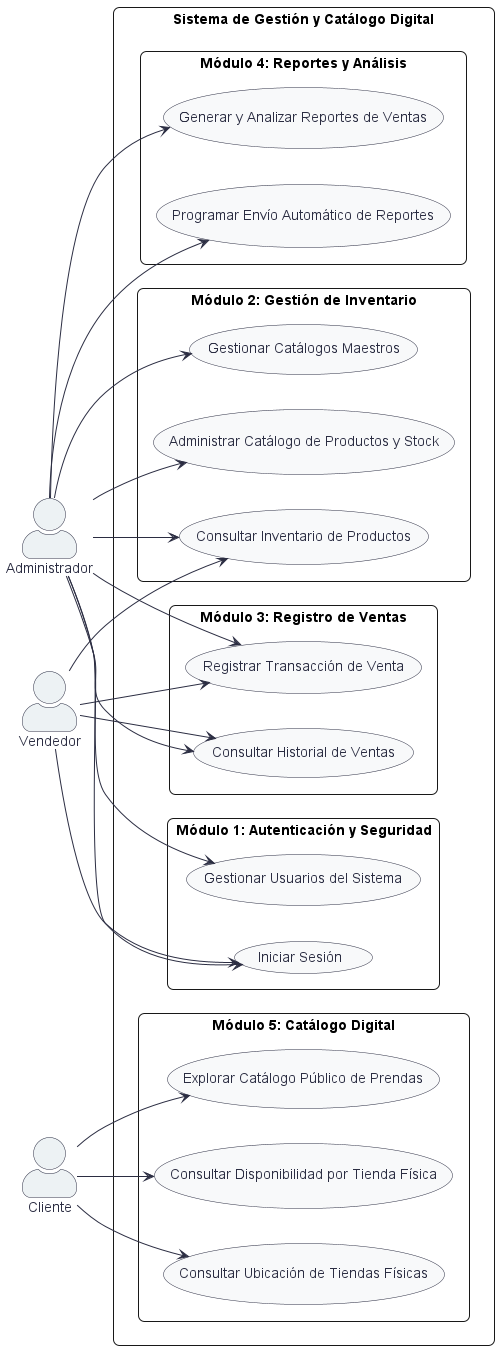
\includegraphics[width=0.92\textwidth]{cu_general_sistema.png}
\caption{Diagrama General de Casos de Uso del Sistema SYSELL Web (UML 2.5)}
\label{fig:cu_general}
\end{figure}

\subsection{Diagramas de Casos de Uso por Módulo Funcional}
A fin de asegurar máxima legibilidad y especificidad técnica, cada módulo funcional cuenta con su respectivo diagrama de interacción UML:

\begin{figure}[H]
\centering
\begin{minipage}{0.48\textwidth}
    \centering
    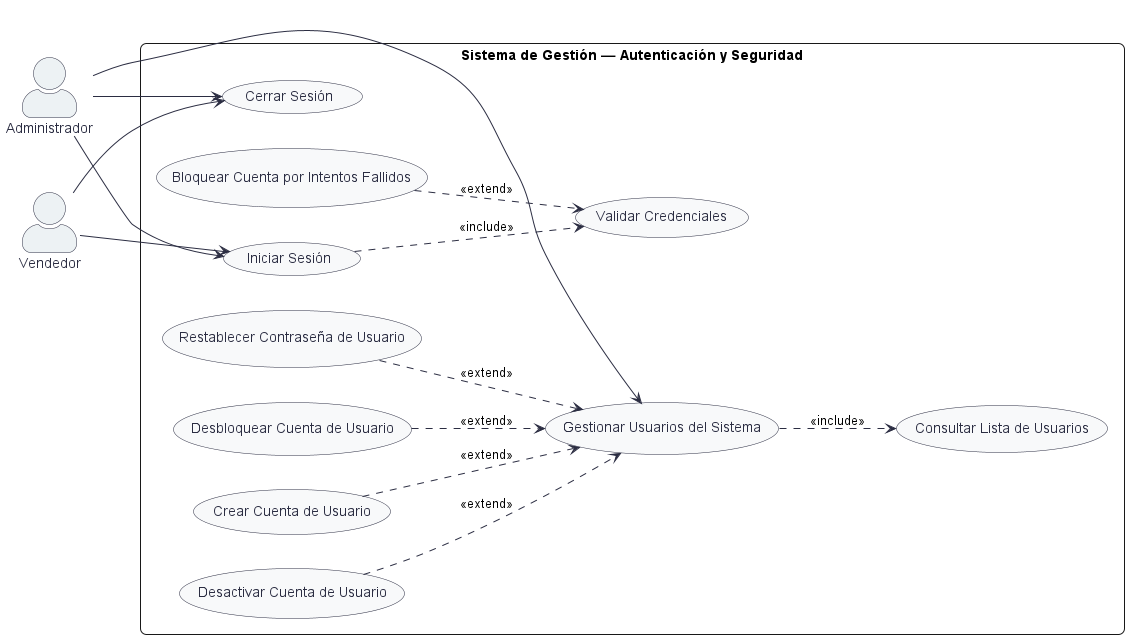
\includegraphics[width=\textwidth]{cu_modulo_1_autenticacion.png}
    \caption{Casos de Uso: Módulo 1 (Autenticación)}
    \label{fig:cu_m1}
\end{minipage}
\hfill
\begin{minipage}{0.48\textwidth}
    \centering
    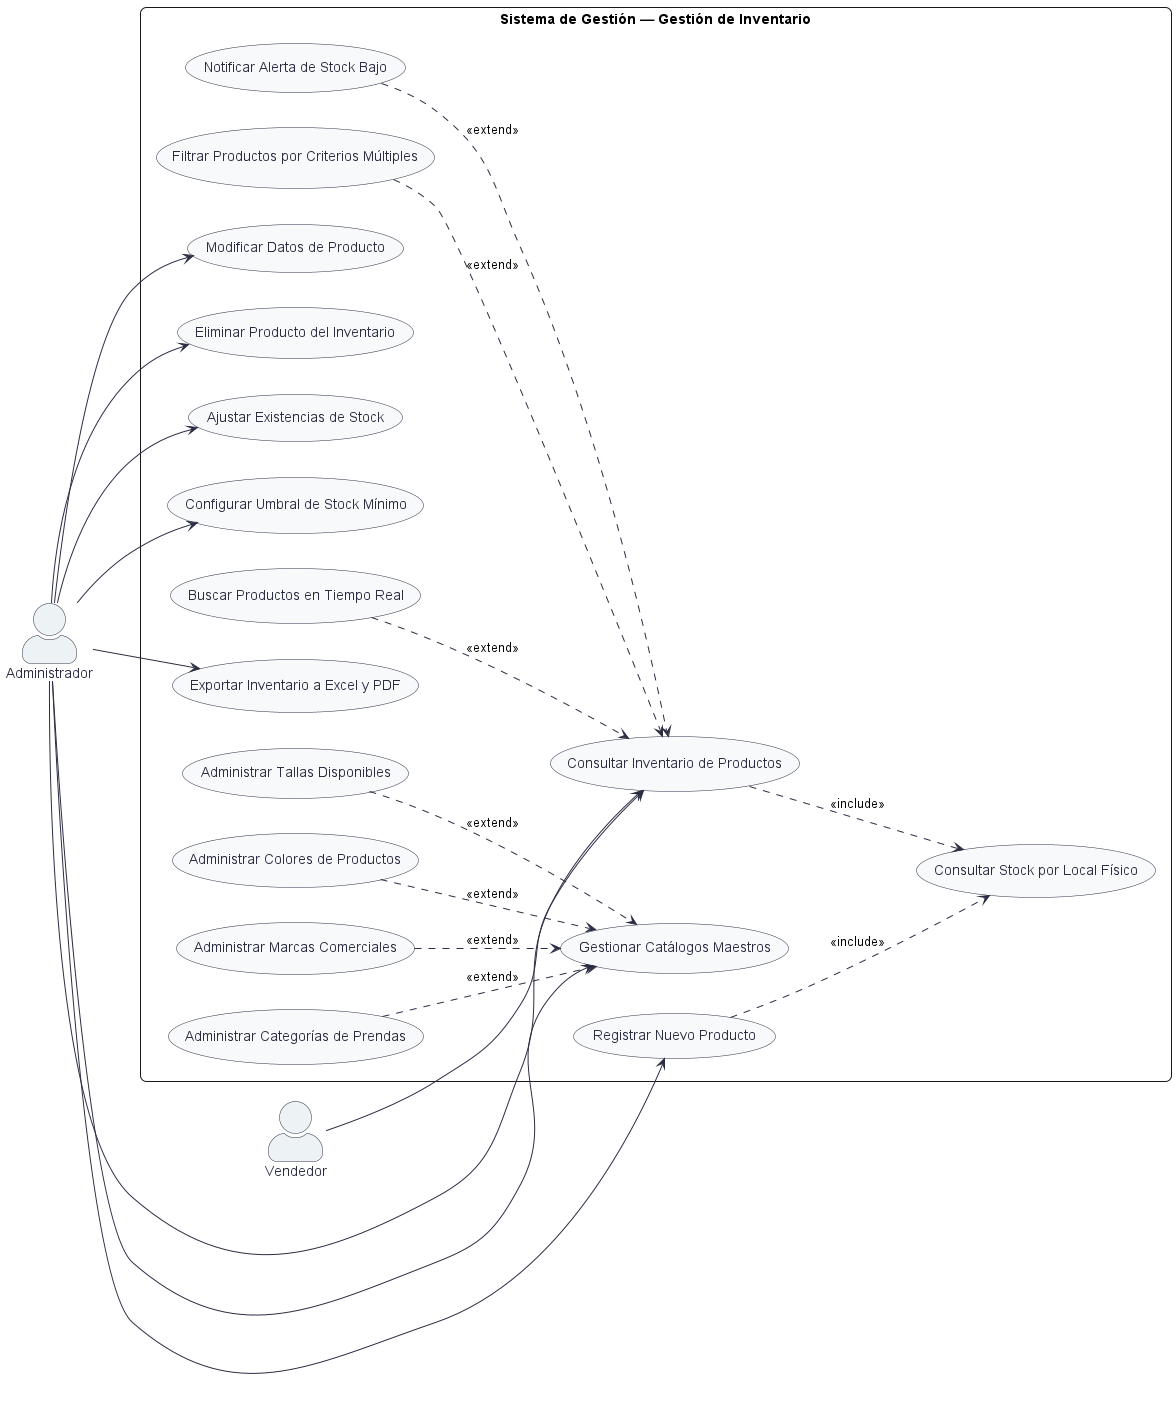
\includegraphics[width=\textwidth]{cu_modulo_2_inventario.png}
    \caption{Casos de Uso: Módulo 2 (Inventario)}
    \label{fig:cu_m2}
\end{minipage}
\end{figure}

\begin{figure}[H]
\centering
\begin{minipage}{0.48\textwidth}
    \centering
    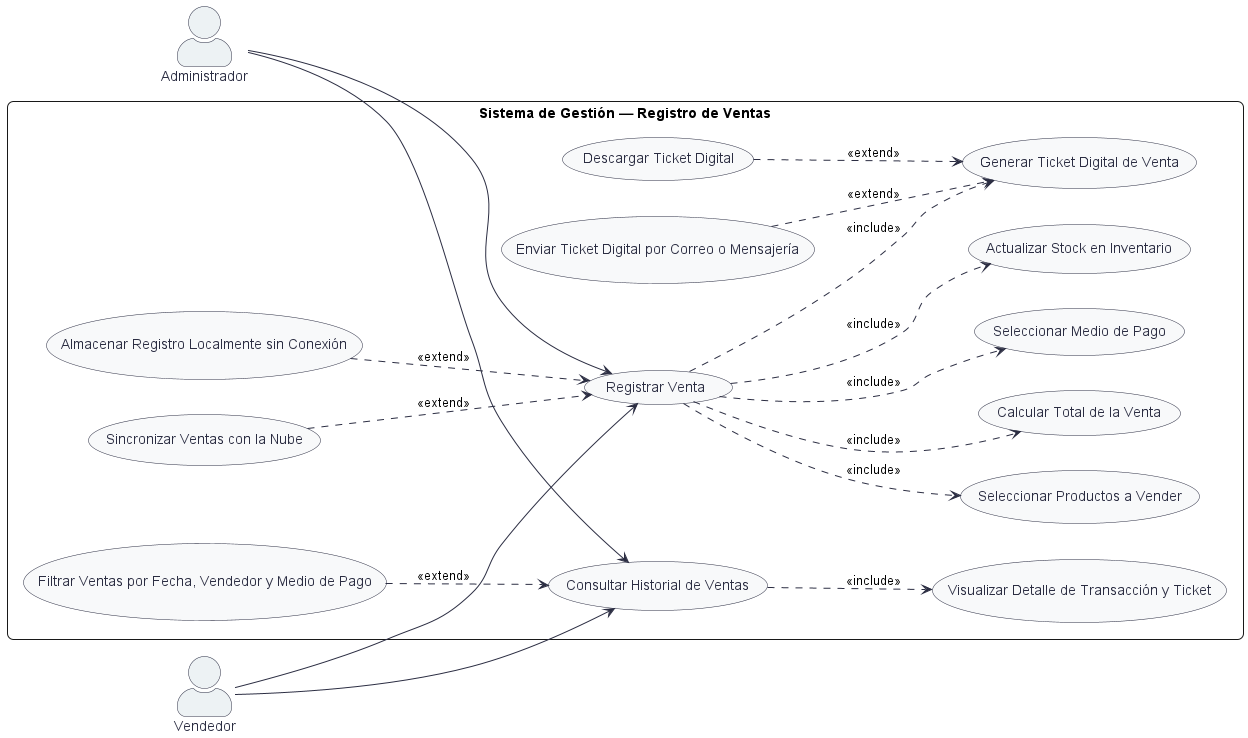
\includegraphics[width=\textwidth]{cu_modulo_3_ventas.png}
    \caption{Casos de Uso: Módulo 3 (Ventas POS)}
    \label{fig:cu_m3}
\end{minipage}
\hfill
\begin{minipage}{0.48\textwidth}
    \centering
    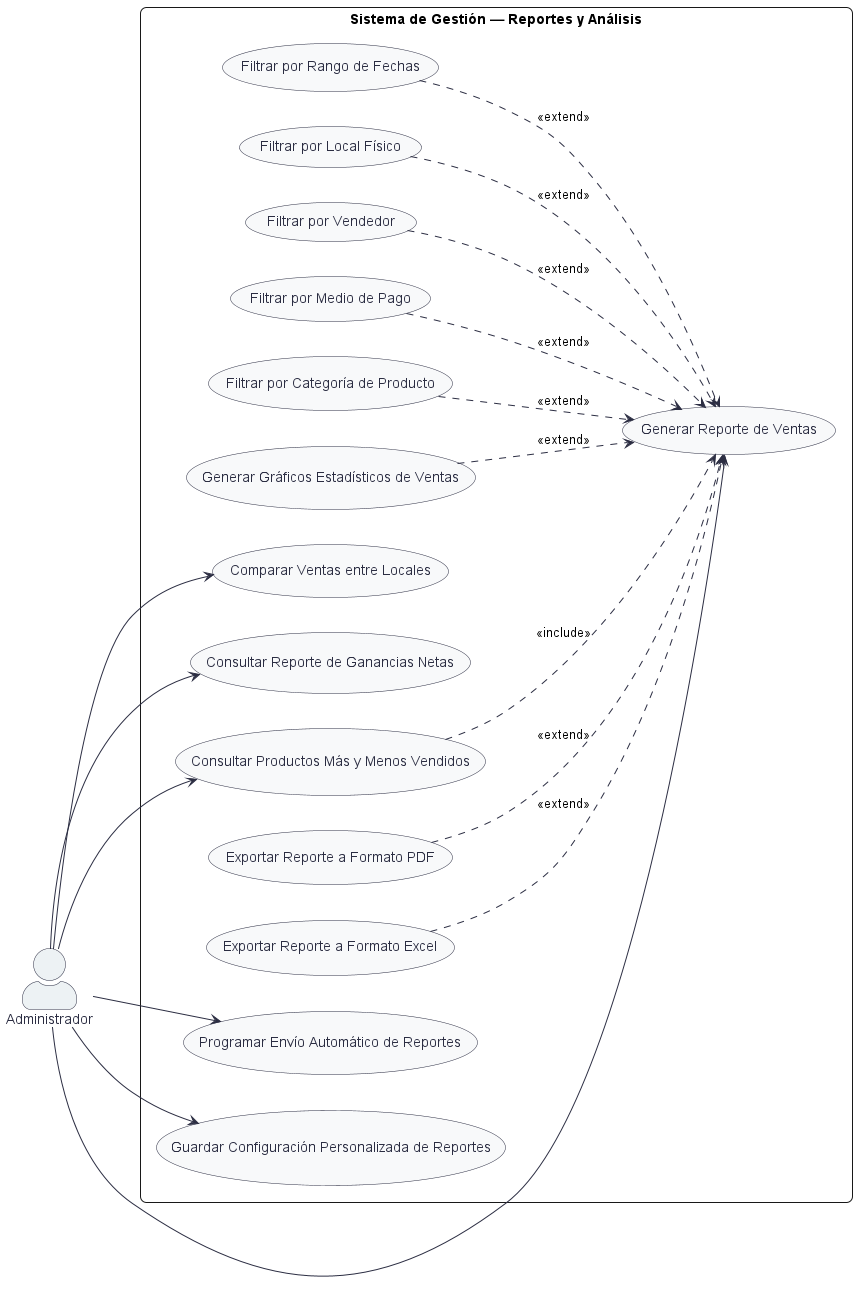
\includegraphics[width=\textwidth]{cu_modulo_4_reportes.png}
    \caption{Casos de Uso: Módulo 4 (Reportes)}
    \label{fig:cu_m4}
\end{minipage}
\end{figure}

\begin{figure}[H]
\centering
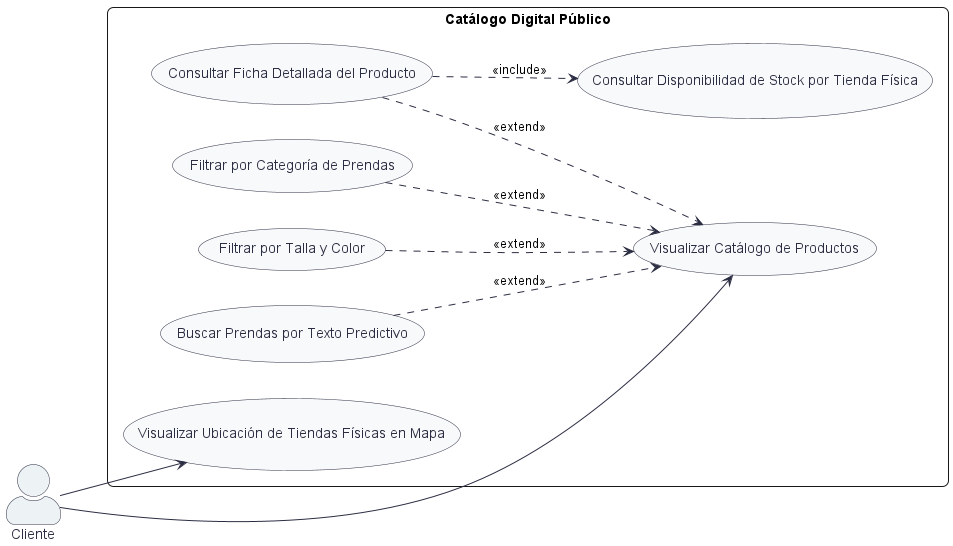
\includegraphics[width=0.6\textwidth]{cu_modulo_5_catalogo.png}
\caption{Casos de Uso: Módulo 5 (Catálogo Digital Público)}
\label{fig:cu_m5}
\end{figure}

\section{Diagramas de Flujo de Datos (DFD) Balanceados}
Para garantizar la consistencia en el tránsito de la información, se modeló el flujo de datos en tres niveles de abstracción balanceados conforme a la metodología de Yourdon/DeMarco:

\subsection{DFD Nivel 0: Diagrama de Contexto}
Delimita las fronteras del sistema informático e identifica los flujos esenciales con las entidades externas:

\begin{figure}[H]
\centering
\begin{tikzpicture}[
    scale=0.88, every node/.style={transform shape},
    entidad/.style={rectangle, draw=primaryblue!80!black, fill=primaryblue!10, rounded corners=3pt, thick, align=center, minimum width=3.2cm, minimum height=1.1cm, font=\small},
    proceso/.style={circle, draw=darkblue, fill=blue!15, line width=1.5pt, align=center, minimum size=3.6cm, font=\small\bfseries},
    dfdArrow/.style={thick, -{Stealth[length=2.2mm]}, primaryblue}
]
\node[proceso] (p0) at (0, 0) {0\\Sistema Web de\\Gestión SYSELL\\(Tienda Machi's)};

\node[entidad, draw=red!70!black, fill=red!10] (admin) at (0, 3.8) {\textbf{Administrador}\\\scriptsize (Propietario / Gerente)};
\node[entidad, draw=green!70!black, fill=green!10] (vendedor) at (-5.8, 0) {\textbf{Vendedor}\\\scriptsize (Caja / Mostrador)};
\node[entidad, draw=orange!70!black, fill=orange!10] (cliente) at (5.8, 0) {\textbf{Cliente Web}\\\scriptsize (Público Comprador)};

% Flujos Vendedor
\draw[dfdArrow] (vendedor.north east) -- node[midway, above=2pt, sloped, font=\scriptsize] {Credenciales, Ventas, Pagos} (p0.north west);
\draw[dfdArrow] (p0.south west) -- node[midway, below=2pt, sloped, font=\scriptsize] {Tickets, Vuelto, Stock local} (vendedor.south east);

% Flujos Administrador
\draw[dfdArrow] (admin.south west) -- node[midway, left=2pt, font=\scriptsize] {Parámetros, Catálogos, Ajustes} (p0.north west);
\draw[dfdArrow] (p0.north east) -- node[midway, right=2pt, font=\scriptsize] {Reportes, Alertas stock, Auditoría} (admin.south east);

% Flujos Cliente Web
\draw[dfdArrow] (cliente.north west) -- node[midway, above=2pt, sloped, font=\scriptsize] {Filtros y búsquedas web} (p0.north east);
\draw[dfdArrow] (p0.south east) -- node[midway, below=2pt, sloped, font=\scriptsize] {Catálogo HD, Disponibilidad tienda} (cliente.south west);

\end{tikzpicture}
\caption{Diagrama de Flujo de Datos: Nivel 0 (Diagrama de Contexto)}
\label{fig:dfd_nivel_0}
\end{figure}

\subsection{DFD Nivel 1: Procesos Principales del Sistema}
Descompone el sistema en cinco procesos macro interconectados con los cinco almacenes de datos normalizados:

\begin{figure}[H]
\centering
\begin{tikzpicture}[
    scale=0.82, every node/.style={transform shape},
    proceso/.style={circle, draw=primaryblue!80!black, fill=primaryblue!10, thick, align=center, minimum size=2.2cm, font=\scriptsize\bfseries},
    almacen/.style={rectangle, draw=purple!80!black, fill=purple!10, rounded corners=2pt, thick, align=center, minimum width=2.8cm, minimum height=0.7cm, font=\scriptsize},
    entidad/.style={rectangle, draw=darkblue, fill=blue!10, rounded corners=2pt, thick, align=center, minimum width=2.6cm, minimum height=0.8cm, font=\scriptsize\bfseries},
    flow/.style={thick, -{Stealth[length=2mm]}, primaryblue}
]
% Entidades
\node[entidad, fill=red!10, draw=red!70!black] (eAdmin) at (-5.5, 3.5) {Administrador};
\node[entidad, fill=green!10, draw=green!70!black] (eVend) at (0, 3.5) {Vendedor};
\node[entidad, fill=orange!10, draw=orange!70!black] (eCli) at (5.5, 3.5) {Cliente Web};

% Procesos
\node[proceso] (p1) at (-4.5, 1.2) {1.0\\Autenticar\\y Usuarios};
\node[proceso] (p2) at (-1.5, 1.2) {2.0\\Gestionar\\Inventario};
\node[proceso] (p3) at (1.5, 1.2) {3.0\\Procesar\\Ventas POS};
\node[proceso] (p4) at (-3, -1.8) {4.0\\Generar\\Reportes};
\node[proceso] (p5) at (4.5, 1.2) {5.0\\Catálogo\\Digital Web};

% Almacenes
\node[almacen] (d1) at (-4.5, -0.2) {D1: Usuarios y Roles};
\node[almacen] (d2) at (-0.5, -0.2) {D2: Catálogos Maestros};
\node[almacen] (d3) at (2.8, -0.2) {D3: Inventario y Kardex};
\node[almacen] (d4) at (0, -1.8) {D4: Ventas y Tickets};
\node[almacen] (d5) at (3.5, -1.8) {D5: Auditoría};

% Conexiones
\draw[flow] (eAdmin) -- (p1);
\draw[flow] (eVend) -- (p1);
\draw[flow] (p1) -- (d1);
\draw[flow] (eAdmin) -- (p2);
\draw[flow] (p2) -- (d2);
\draw[flow] (p2) -- (d3);
\draw[flow] (eVend) -- (p3);
\draw[flow] (p3) -- (d3);
\draw[flow] (p3) -- (d4);
\draw[flow] (p3) -- (d5);
\draw[flow] (eAdmin) -- (p4);
\draw[flow] (d4) -- (p4);
\draw[flow] (eCli) -- (p5);
\draw[flow] (d3) -- (p5);

\end{tikzpicture}
\caption{Diagrama de Flujo de Datos: Nivel 1 (Procesos Principales y Almacenes D1--D5)}
\label{fig:dfd_nivel_1}
\end{figure}

\subsection{DFD Nivel 2: Descomposición del Proceso de Ventas (P 3.0)}
Desglosa la lógica transaccional de caja en cinco subprocesos atómicos:

\begin{figure}[H]
\centering
\begin{tikzpicture}[
    scale=0.85, every node/.style={transform shape},
    subproc/.style={circle, draw=primaryblue!80!black, fill=primaryblue!10, thick, align=center, minimum size=1.9cm, font=\scriptsize\bfseries},
    store/.style={rectangle, draw=purple!80!black, fill=purple!10, rounded corners=2pt, thick, align=center, minimum width=2.6cm, minimum height=0.6cm, font=\scriptsize},
    flow/.style={thick, -{Stealth[length=2mm]}, primaryblue}
]
\node[subproc] (p31) at (0, 0) {3.1\\Validar Stock\\y Prenda};
\node[subproc] (p32) at (3.0, 0) {3.2\\Calcular\\Totales};
\node[subproc] (p33) at (6.0, 0) {3.3\\Registrar\\Cobro};
\node[subproc] (p34) at (9.0, 0) {3.4\\Actualizar\\Inventario};
\node[subproc] (p35) at (12.0, 0) {3.5\\Emitir\\Ticket};

\node[store] (d3) at (0, -1.8) {D3: Inventario};
\node[store] (d4) at (12.0, -1.8) {D4: Ventas};
\node[store] (d5) at (9.0, -1.8) {D5: Kardex};

\draw[flow] (p31) -- (p32);
\draw[flow] (p32) -- (p33);
\draw[flow] (p33) -- (p34);
\draw[flow] (p34) -- (p35);

\draw[flow] (d3) -- (p31);
\draw[flow] (p34) -- (d3);
\draw[flow] (p34) -- (d5);
\draw[flow] (p35) -- (d4);

\end{tikzpicture}
\caption{Diagrama de Flujo de Datos: Nivel 2 (Descomposición del Proceso de Ventas 3.0)}
\label{fig:dfd_nivel_2}
\end{figure}

\section{Diccionario de Almacenes de Datos Normalizados (D1 a D5)}
\begin{table}[H]
\centering
\small
\begin{tabularx}{\textwidth}{>{\ttfamily\centering}p{1.2cm} >{\raggedright\bfseries}p{3.8cm} >{\ttfamily\small\raggedright}p{4cm} Y}
\toprule
\textbf{Almacén} & \textbf{Nombre del Almacén} & \textbf{Tablas Relacionales Asociadas} & \textbf{Contenido y Finalidad} \\
\midrule
D1 & Usuarios y Roles & usuarios, locales & Cuentas, credenciales Bcrypt, roles RBAC y asignación física de locales. \\
\addlinespace
D2 & Catálogos Maestros & categorias, marcas, tallas, colores & Listas cerradas inmutables para selección de atributos de prendas (RF-74). \\
\addlinespace
D3 & Inventario y Kardex & productos, variantes\_producto, inventario, ajustes\_inventario & Existencias por tienda, SKUs normalizados, alertas de stock y auditoría de Kardex. \\
\addlinespace
D4 & Ventas y Comprobantes & ventas, detalle\_ventas, pagos\_venta, metodos\_pago & Encabezados, desglose de prendas vendidas, importes, medios mixtos y tickets. \\
\addlinespace
D5 & Bitácora y Auditoría & auditoria, reportes\_configuracion & Registro inmutable de eventos críticos (crear, anular, resetear) con detalle JSON. \\
\bottomrule
\end{tabularx}
\caption{Mapeo formal de almacenes de datos DFD a tablas de la base de datos MySQL}
\label{tab:almacenes_dfd}
\end{table}
